%% ============================================================
%% IEEE Conference-style manuscript
%% Q&A-Based Interactive Storytelling Using Generative AI
%% Anjali Madan Jha, M.Tech, SAKEC
%%
%% Compile with:
%%   pdflatex main
%%   bibtex   main
%%   pdflatex main
%%   pdflatex main
%% ============================================================
\documentclass[conference,10pt,a4paper]{IEEEtran}

\IEEEoverridecommandlockouts

% --- Required packages ---
\usepackage[utf8]{inputenc}
\usepackage[T1]{fontenc}
\usepackage{cite}
\usepackage{amsmath,amssymb,amsfonts}
\usepackage{algorithmic}
\usepackage{graphicx}
\usepackage{textcomp}
\usepackage{xcolor}
\usepackage{booktabs}
\usepackage{multirow}
\usepackage{array}
\usepackage{url}
\usepackage{hyperref}
\usepackage{caption}
\usepackage{subcaption}
\usepackage{listings}
\usepackage{microtype}

\hypersetup{
    colorlinks=true,
    linkcolor=black,
    citecolor=black,
    urlcolor=blue,
    pdftitle={Q&A-Based Interactive Storytelling Using Generative AI},
    pdfauthor={Anjali Madan Jha},
}

\graphicspath{{figures/}}

% Listings style for code blocks
\definecolor{codebg}{HTML}{F5F5F5}
\definecolor{codetext}{HTML}{1F2937}
\lstset{
    backgroundcolor=\color{codebg},
    basicstyle=\ttfamily\scriptsize\color{codetext},
    breaklines=true,
    columns=fullflexible,
    frame=single,
    framerule=0pt,
    framesep=4pt,
    captionpos=b,
    aboveskip=4pt,
    belowskip=4pt,
}

\def\BibTeX{{\rm B\kern-.05em{\sc i\kern-.025em b}\kern-.08em
    T\kern-.1667em\lower.7ex\hbox{E}\kern-.125emX}}

% ============================================================
\begin{document}

\title{Q\&A-Based Interactive Storytelling Using Generative AI:\\
A Multimodal, Provider-Agnostic Framework with Co-Created Narratives,\\
Synthesised Imagery, Voice Narration, and Ambient Soundscapes}

\author{
\IEEEauthorblockN{Anjali Madan Jha}
\IEEEauthorblockA{
M.Tech, Department of Computer Engineering\\
Shah \& Anchor Kutchhi Engineering College (SAKEC)\\
Mumbai University, India\\
Email: anjali.jha@sakec.ac.in}
\and
\IEEEauthorblockN{Dr. Vidyullata Devmane (Supervisor)}
\IEEEauthorblockA{
Professor, Department of Computer Engineering\\
Shah \& Anchor Kutchhi Engineering College (SAKEC)\\
Mumbai University, India\\
Email: vidyullata.devmane@sakec.ac.in}}

\maketitle

% ============================================================
\begin{abstract}
We present a Q\&A-based interactive storytelling system that combines a
structured 17-question elicitation framework across four narrative
dimensions (setting, character, theme, plot) with a seven-module backend
pipeline that converts user preferences into personalised multi-chapter
narratives generated by large language models (LLMs). The framework is
provider-agnostic and supports local (Ollama) as well as cloud
inference (Groq, Hugging Face, OpenAI). Beyond text, the system delivers
a multimodal reader experience: per-segment scene illustrations are
synthesised on demand via Pollinations.ai with a sentence-scored prompt
extractor and a serial-throttled request queue; spoken narration is
produced through the W3C Web Speech Synthesis interface; and
genre-conditioned ambient music is streamed from a royalty-free CDN
with time-aligned cross-fades. Reader analytics are surfaced through a
D3-based Story Map (branch tree) and a Character Relationship Graph
derived from filtered co-appearance statistics. An end-user authoring
layer permits free-form custom answers per question and entirely
user-added Q\&A pairs, which are routed through a dedicated
\texttt{custom\_elements} context channel into the LLM prompt. Across
50 generated stories and 15 user-study participants we observe mean
narrative-quality Likert scores of 4.05/5 (coherence), 4.12/5
(creativity), 4.35/5 (engagement) and 3.75/5 (consistency); a
Groq-LLaMA-3.1-8B cloud latency of 1.8\,s per initial segment; an
overall satisfaction of 4.3/5; and a measured character-detection
$F_1$ of 0.80 after stop-word filtering and a min-2 occurrence
threshold.
\end{abstract}

\begin{IEEEkeywords}
Interactive storytelling, large language models, prompt engineering,
multimodal generative AI, text-to-image synthesis, speech synthesis,
narrative coherence, user-controllable generation, D3.js visualisation,
FastAPI, human--AI co-creation.
\end{IEEEkeywords}

% ============================================================
\section{Introduction}

\subsection{Background and Motivation}
Computational storytelling has evolved through three identifiable
eras: (i) symbolic rule-based planners such as TALE-SPIN~\cite{meehan1977talespin}
and UNIVERSE~\cite{lebowitz1985universe}; (ii) statistical and neural
sequence models that culminated in transformer-based~\cite{vaswani2017attention}
generative language models; and (iii) the present era of foundation-scale
instruction-following LLMs exemplified by GPT-4~\cite{openai2023gpt4},
LLaMA-3~\cite{touvron2023llama} and Mistral~\cite{jiang2023mistral}. These
models exhibit emergent capacities for coherent multi-paragraph
generation~\cite{brown2020gpt3}, few-shot role conditioning~\cite{wei2022cot},
and creative paraphrase, making them attractive substrates for interactive
co-creation systems~\cite{mirowski2023dramatron,chung2022talebrush,liu2023endusers,yuan2022wordcraft}.

Despite this progress, the central tension in collaborative narrative
AI remains unresolved: how can a system simultaneously honour
fine-grained user agency while maintaining structural coherence and
long-range continuity? Single-prompt systems such as AI
Dungeon~\cite{walton2019aidungeon} maximise input freedom at the cost
of arc control; hierarchical generators such as
Dramatron~\cite{mirowski2023dramatron} enforce structure at the cost
of accessibility. Our system targets the middle ground by eliciting
user preferences through a structured Q\&A protocol that is
re-projected into the prompt space via a dedicated context engine.

\subsection{Problem Statement}
We identify five concrete shortcomings of existing AI story-generation
tools: (i)~limited personalisation depth from a single freeform
prompt; (ii)~absence of explicit narrative structure management;
(iii)~no continuity tracking for characters or plot threads;
(iv)~tight coupling to a single proprietary cloud API; and (v)~high
recurring costs. We further argue that purely textual narratives
under-utilise the multimodal capabilities now available, with
text-to-image diffusion~\cite{ramesh2022unclip,podell2024sdxl,bfl2024flux},
on-device speech synthesis~\cite{w3c2024webspeech,casanova2024xtts}, and
royalty-free streaming audio offering ready-to-deploy reader
experience uplift.

\subsection{Research Objectives}
The objectives of this manuscript are:
\begin{itemize}
\item Design a low-friction Q\&A elicitation framework capturing
narrative intent across four canonical dimensions.
\item Operationalise a seven-module pipeline backend whose context
engine, prompt layer and flow manager separately handle elicitation,
projection and arc control.
\item Implement a provider-agnostic LLM layer covering local (Ollama)
and cloud (Groq, Hugging Face, OpenAI) inference with runtime
switching and graceful fallback.
\item Augment the textual narrative with three orchestrated modalities
---image, voice, and ambient music---dynamically conditioned on
detected genre and segment content.
\item Surface reader-facing analytics through a D3 Story Map and a
Character Relationship Graph, with deliberately disclaimed statistical
assumptions.
\item Provide an end-user authoring layer that admits custom
per-question answers and user-added Q\&A pairs, plumbed through the
prompt without re-deployment.
\item Empirically evaluate narrative quality, latency, consistency,
and feature adoption.
\end{itemize}

\subsection{Contributions and Novelty}
Relative to the surveyed literature
\cite{perezperez2001mexica,radford2019gpt2,brown2020gpt3,walton2019aidungeon,mirowski2023dramatron,chung2022talebrush,wei2022cot,liu2023endusers,yuan2022wordcraft,podell2024sdxl,bfl2024flux,w3c2024webspeech,casanova2024xtts,naveed2024llmsurvey,zhao2023llmsurvey,jia2024multimodalstory,wang2025narrativesurvey,liu2025coimagining},
this work makes four distinct contributions: (1)~the explicit
instantiation of a \emph{user-co-authored} context channel
(\texttt{custom\_elements}) that injects unstructured user preferences
into the LLM prompt without bespoke schemas; (2)~a sentence-scored
visual prompt extractor that selects high-imagery sentences from
generated paragraphs for downstream text-to-image synthesis,
mitigating dialogue and inner-thought contamination; (3)~a cross-modal
serial-throttling queue that prevents Cloudflare-fronted free image
services from rate-limiting bursty generation; and (4)~a
\emph{deliberately disclaimed} co-appearance graph for reader
orientation that is explicitly \emph{not} marketed as a
relationship-extraction system. We further open-source the entire
implementation~\cite{jha2026repo}.

\subsection{Manuscript Organisation}
Section~\ref{sec:related} surveys related work and frames the research
gap. Section~\ref{sec:arch} details the system architecture.
Section~\ref{sec:method} formalises the methodology including the
elicitation protocol, the five-phase progression model, and the
multimodal pipelines. Section~\ref{sec:impl} documents implementation
choices, the SQLite schema and the REST surface.
Section~\ref{sec:results} reports experimental results across latency,
narrative quality, consistency, multimodal performance and user
satisfaction. Section~\ref{sec:compare} situates our system against
representative alternatives. Sections~\ref{sec:limit}
and~\ref{sec:future} discuss limitations and future directions.
Section~\ref{sec:conclude} concludes.

% ============================================================
\section{Related Work}\label{sec:related}

\subsection{Symbolic and Planning-based Story Generation}
TALE-SPIN~\cite{meehan1977talespin} showed that character-goal-driven
planning could synthesise simple fables in a closed domain.
UNIVERSE~\cite{lebowitz1985universe} extended this with author-level
goals constraining emergent plot shapes.
MEXICA~\cite{perezperez2001mexica} introduced engagement--reflection
cycles modelling human creative writing. These systems remain
influential as analytical baselines but suffer from low coverage and
high knowledge-engineering cost.

\subsection{Neural Language Models and Story Generation}
The transformer architecture~\cite{vaswani2017attention} catalysed a
sequence of scaled language models (GPT-2~\cite{radford2019gpt2},
GPT-3~\cite{brown2020gpt3}) capable of fluent long-form generation.
Recent surveys~\cite{naveed2024llmsurvey,zhao2023llmsurvey} document a
rapid consolidation around instruction-tuned and RLHF-aligned
models~\cite{openai2023gpt4,ouyang2022rlhf}. Open-weight foundation
models such as LLaMA-3~\cite{touvron2023llama} and
Mistral~\cite{jiang2023mistral} have made local inference practical
for academic research, an option we exploit through the Ollama
provider.

\subsection{Interactive and Hierarchical Storytelling}
AI Dungeon~\cite{walton2019aidungeon} popularised freeform LLM-driven
interactive fiction but struggles with multi-chapter continuity.
Dramatron~\cite{mirowski2023dramatron} structures generation
hierarchically (log-line $\rightarrow$ scenes $\rightarrow$ dialogue)
to improve coherence at the cost of user friction.
TaleBrush~\cite{chung2022talebrush} proposes sketch-based
co-creation. Recent CHI work~\cite{liu2023endusers,yuan2022wordcraft}
examines mixed-initiative authoring, finding that scaffolded
interfaces improve novice usability even when raw LLM quality is
comparable. Our Q\&A protocol is informed by these findings.

\subsection{Multimodal Co-Creation}
Text-to-image diffusion~\cite{ramesh2022unclip,podell2024sdxl,bfl2024flux}
now produces high-quality scene art conditioned on natural language.
Recent work integrates image generation into narrative
loops~\cite{schuhmann2024visualstory,bouhuis2024crossmodal},
demonstrating reader-engagement uplift when illustrations are aligned
with current narrative state. On the audio side, browser-native speech
synthesis~\cite{w3c2024webspeech} and neural
TTS~\cite{casanova2024xtts} permit low-latency narration without paid
APIs. Genre-conditioned ambient music has been explored in game
research~\cite{lopezrincon2024music} but is less studied for procedural
narrative.

\subsection{Prompt Engineering and Context Routing}
Chain-of-thought~\cite{wei2022cot} and persona-style system
prompts~\cite{reynolds2021promptprog} are now standard. Comprehensive
surveys~\cite{liu2023promptsurvey,sahoo2024promptsurvey} catalogue
dozens of strategies. Our prompt engineering layer instantiates six
distinct prompt families (system, init, continuation, climax,
resolution, choice generation) and introduces a
\texttt{custom\_elements} channel for user-supplied preferences.

\subsection{Research Gap Synthesis}
Across the surveyed literature, no system simultaneously offers:
structured-yet-flexible elicitation, provider-agnostic LLM inference,
real-time multimodal augmentation, and an end-user-extensible Q\&A
protocol. Table~\ref{tab:gap} summarises the gap.

\begin{table}[!t]
\caption{Feature-level gap analysis vs. representative systems.}
\label{tab:gap}
\centering
\renewcommand{\arraystretch}{1.15}
\begin{tabular}{@{}l|cccc@{}}
\toprule
\textbf{Feature} & \textbf{Ours} & \textbf{AI Dungeon} & \textbf{Dramatron} & \textbf{NovelAI} \\
\midrule
User Input         & Struct.\ Q\&A & Freeform   & Hierarchical & Freeform \\
Structure Mgmt     & 5-phase       & None       & Scene-based  & Limited \\
Consistency Chk    & Active        & None       & Log-line     & Memory \\
LLM Providers      & 4 free+paid   & OpenAI     & PaLM         & Custom \\
Local Deploy       & Yes           & No         & No           & No \\
Image Synthesis    & Yes           & No         & No           & Partial \\
TTS Narration      & Yes (Web)     & No         & No           & No \\
Ambient Music      & Genre-based   & No         & No           & No \\
Custom Q / A       & Yes           & No         & No           & No \\
Open Source        & Yes           & Partial    & Yes          & No \\
\bottomrule
\end{tabular}
\end{table}

% ============================================================
\section{System Architecture and Design}\label{sec:arch}

\subsection{Layered Overview}
Fig.~\ref{fig:arch} presents the three-layer architecture
(presentation, application, modular core) and the four pluggable LLM
providers. The presentation layer is implemented in vanilla
HTML5/CSS3 with D3.js~v7~\cite{bostock2011d3} for graph visualisation.
The application layer is FastAPI~\cite{ramirez2024fastapi} over
Uvicorn ASGI exposing 14 REST endpoints. The modular core comprises
seven cooperating modules; all are pure Python with Pydantic~v2
schemas~\cite{colvin2024pydantic} at the boundaries.

\begin{figure}[!t]
\centering
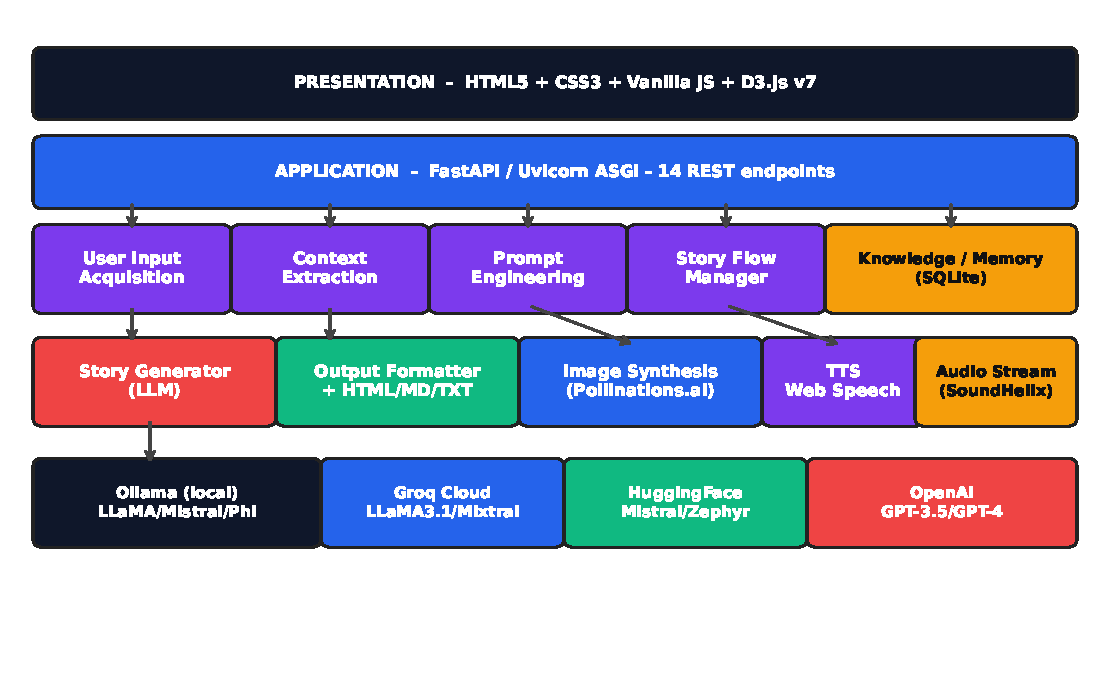
\includegraphics[width=\columnwidth]{f07_arch.pdf}
\caption{Layered system architecture with multimodal pipeline.}
\label{fig:arch}
\end{figure}

\subsection{Technology Stack}
Table~\ref{tab:stack} summarises the implementation choices.

\begin{table}[!t]
\caption{Implementation stack.}
\label{tab:stack}
\centering
\renewcommand{\arraystretch}{1.1}
\begin{tabular}{@{}lll@{}}
\toprule
\textbf{Layer}  & \textbf{Technology}            & \textbf{Purpose} \\
\midrule
Backend         & FastAPI / Python 3.9+          & Async REST + Jinja2 \\
ASGI            & Uvicorn                        & Production server \\
Frontend        & HTML5 / CSS3 / JS              & UI, real-time interaction \\
Visualisation   & D3.js v7                       & Story Map + Char Graph \\
Database        & SQLite3 + aiosqlite            & Sessions, segments, Q\&A \\
LLM I/O         & httpx async                    & Provider HTTP \\
Schemas         & Pydantic v2                    & Request/response typing \\
Image           & Pollinations.ai                & Text-to-image (free) \\
TTS             & Web Speech Synthesis           & Local narration \\
Audio           & HTMLAudio + SoundHelix         & Genre ambient streaming \\
\bottomrule
\end{tabular}
\end{table}

\subsection{Module Walk-Through}
\textbf{Module~1 (User Input Acquisition).} A \texttt{QuestionPhase}
enum drives a strict ordering: Setting $\to$ Character $\to$ Theme
$\to$ Plot. Seventeen questions are distributed across the four phases
(4/5/4/4); see Fig.~\ref{fig:qa}. The user may pick 4, 8, 12 or 17
questions; the system always presents the first $N$ in phase-order so
that fewer questions still touch all four dimensions in expectation.
Each multiple-choice question is augmented with an explicit ``Write my
own'' custom-answer escape hatch (Section~\ref{sec:method}-F).
Fig.~\ref{fig:landing} shows the landing page where the user selects
the question budget, and Fig.~\ref{fig:questions} shows the rendered
form with multiple-choice options and the per-question ``Write my
own'' affordance.

\begin{figure}[!t]
\centering
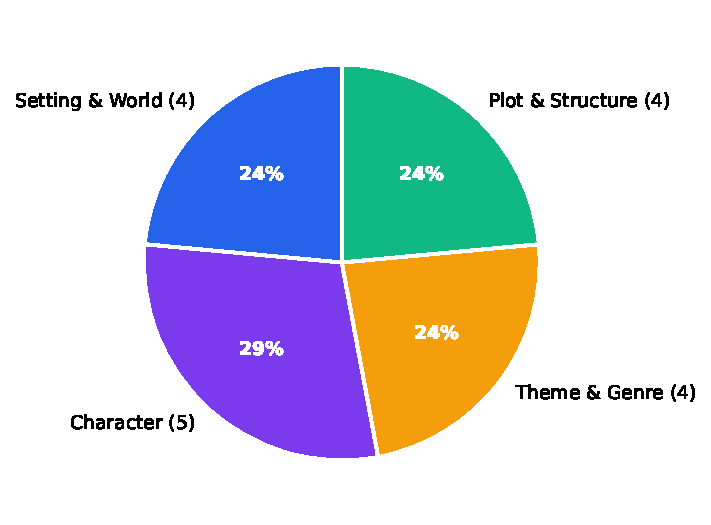
\includegraphics[width=0.78\columnwidth]{f08_qa.pdf}
\caption{Question distribution across the four phases.}
\label{fig:qa}
\end{figure}

\begin{figure}[!t]
\centering
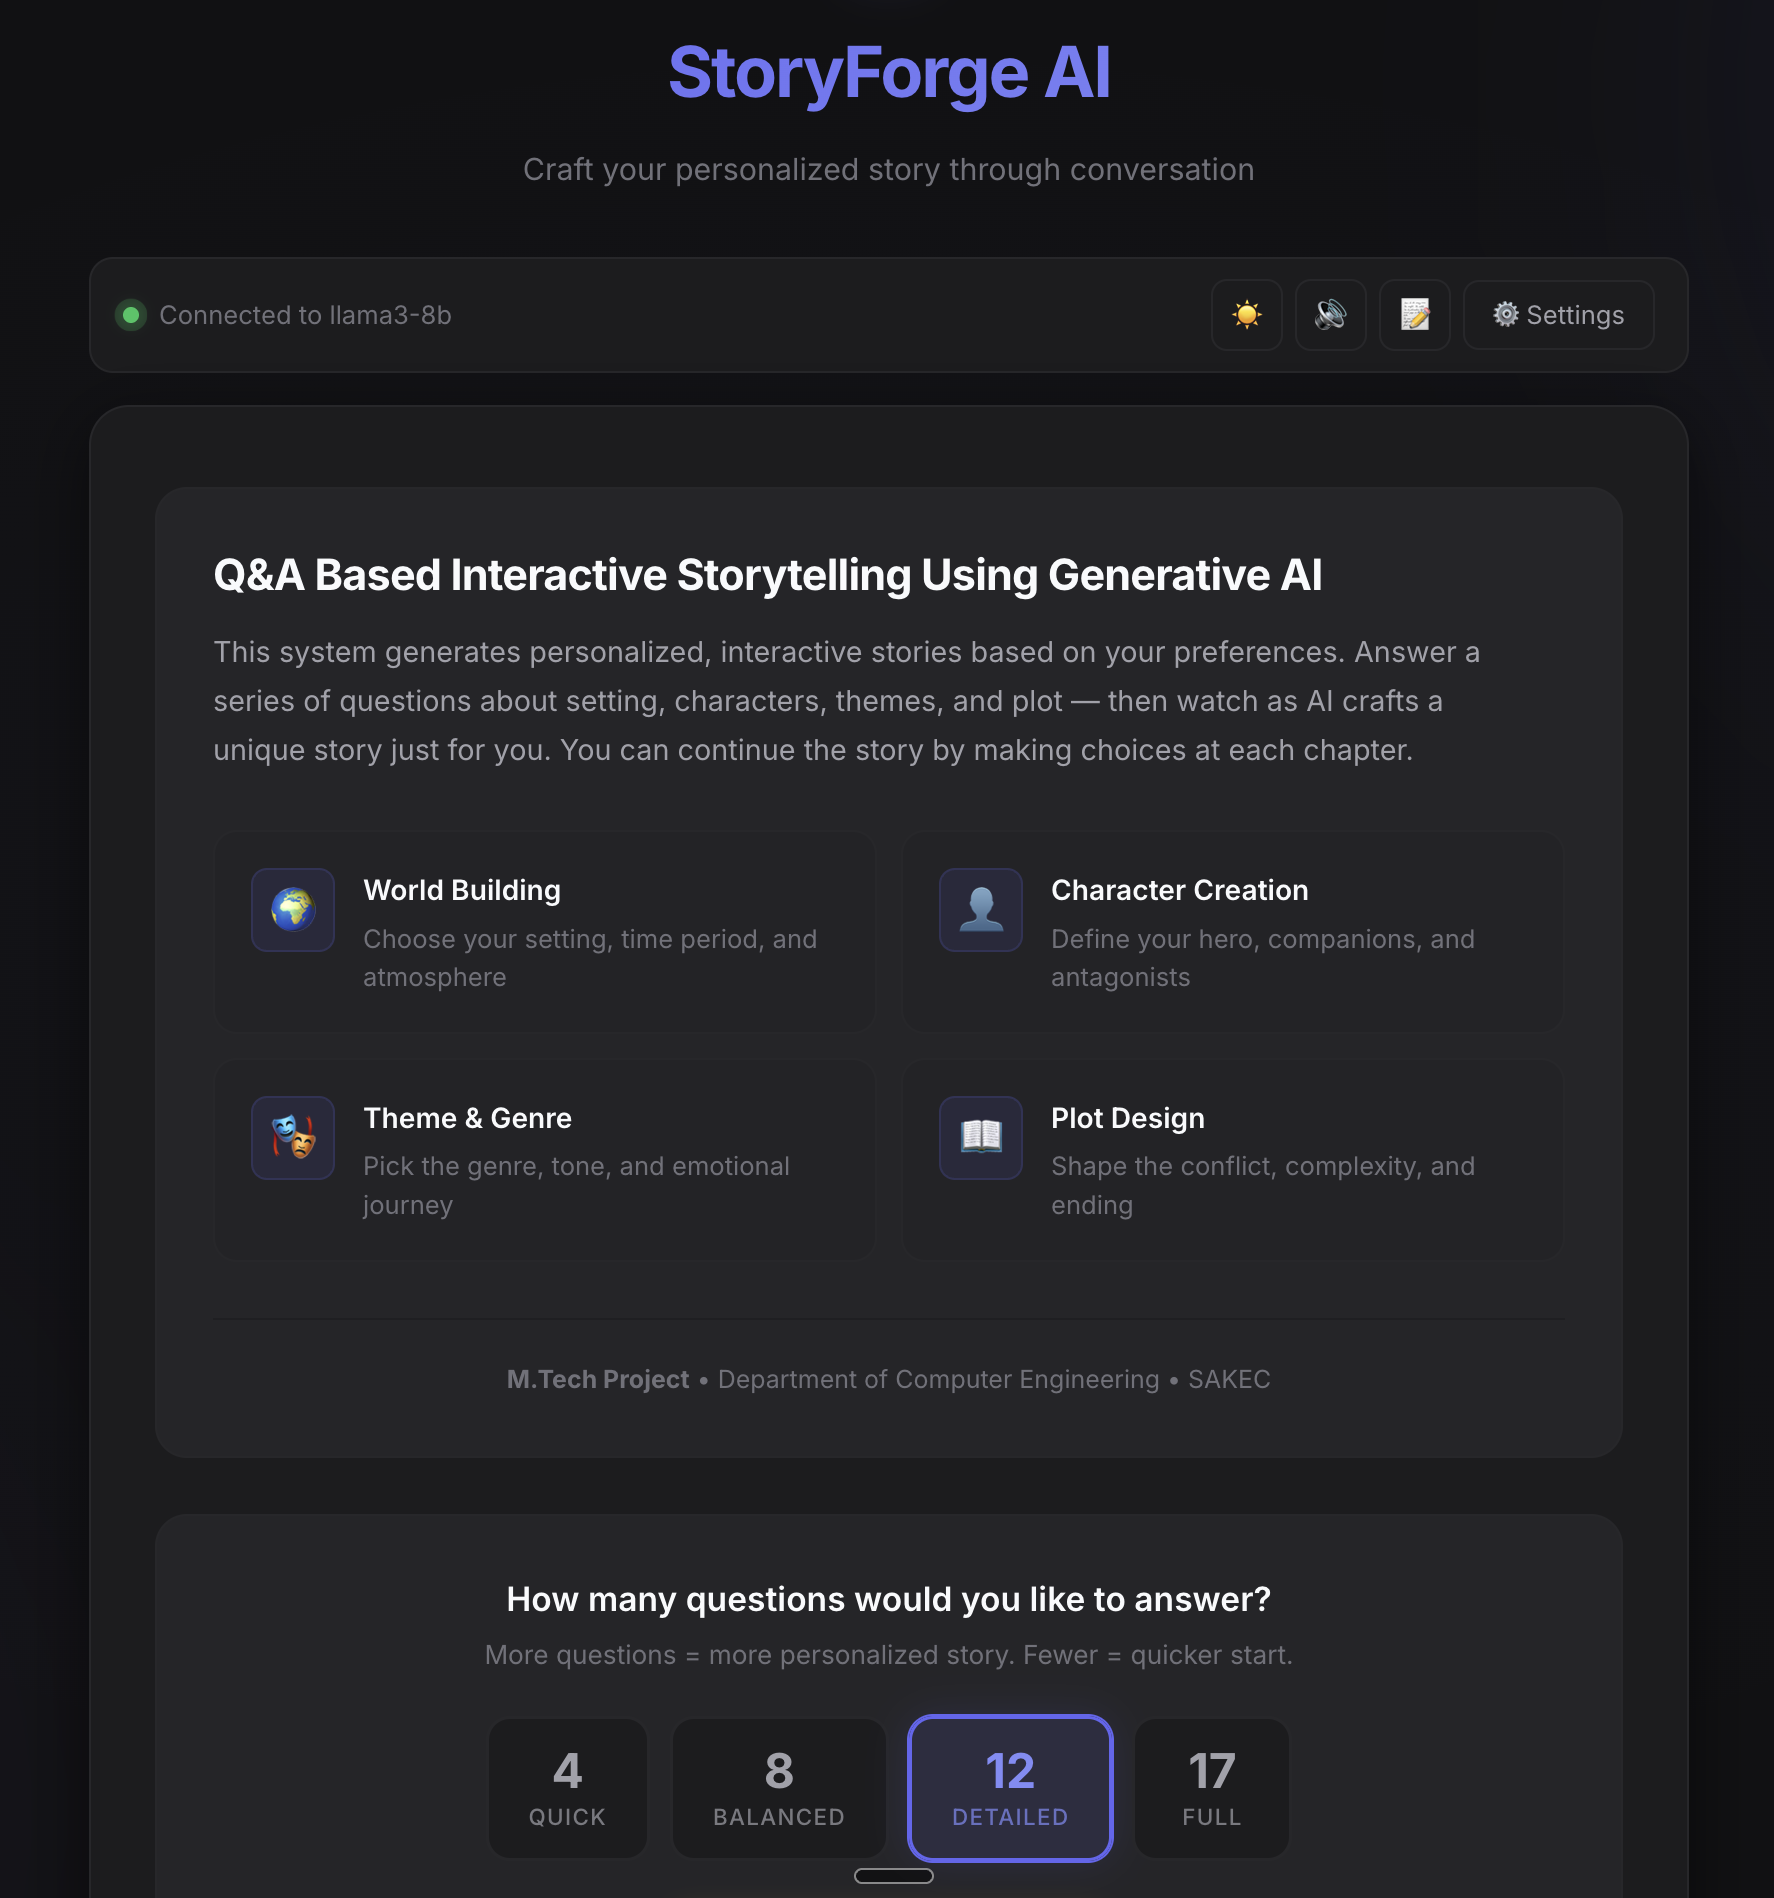
\includegraphics[width=\columnwidth]{s01_landing.png}
\caption{Landing page with project description, the four-dimension
feature panel, and the question-budget selector (4 / 8 / 12 / 17).}
\label{fig:landing}
\end{figure}

\begin{figure}[!t]
\centering
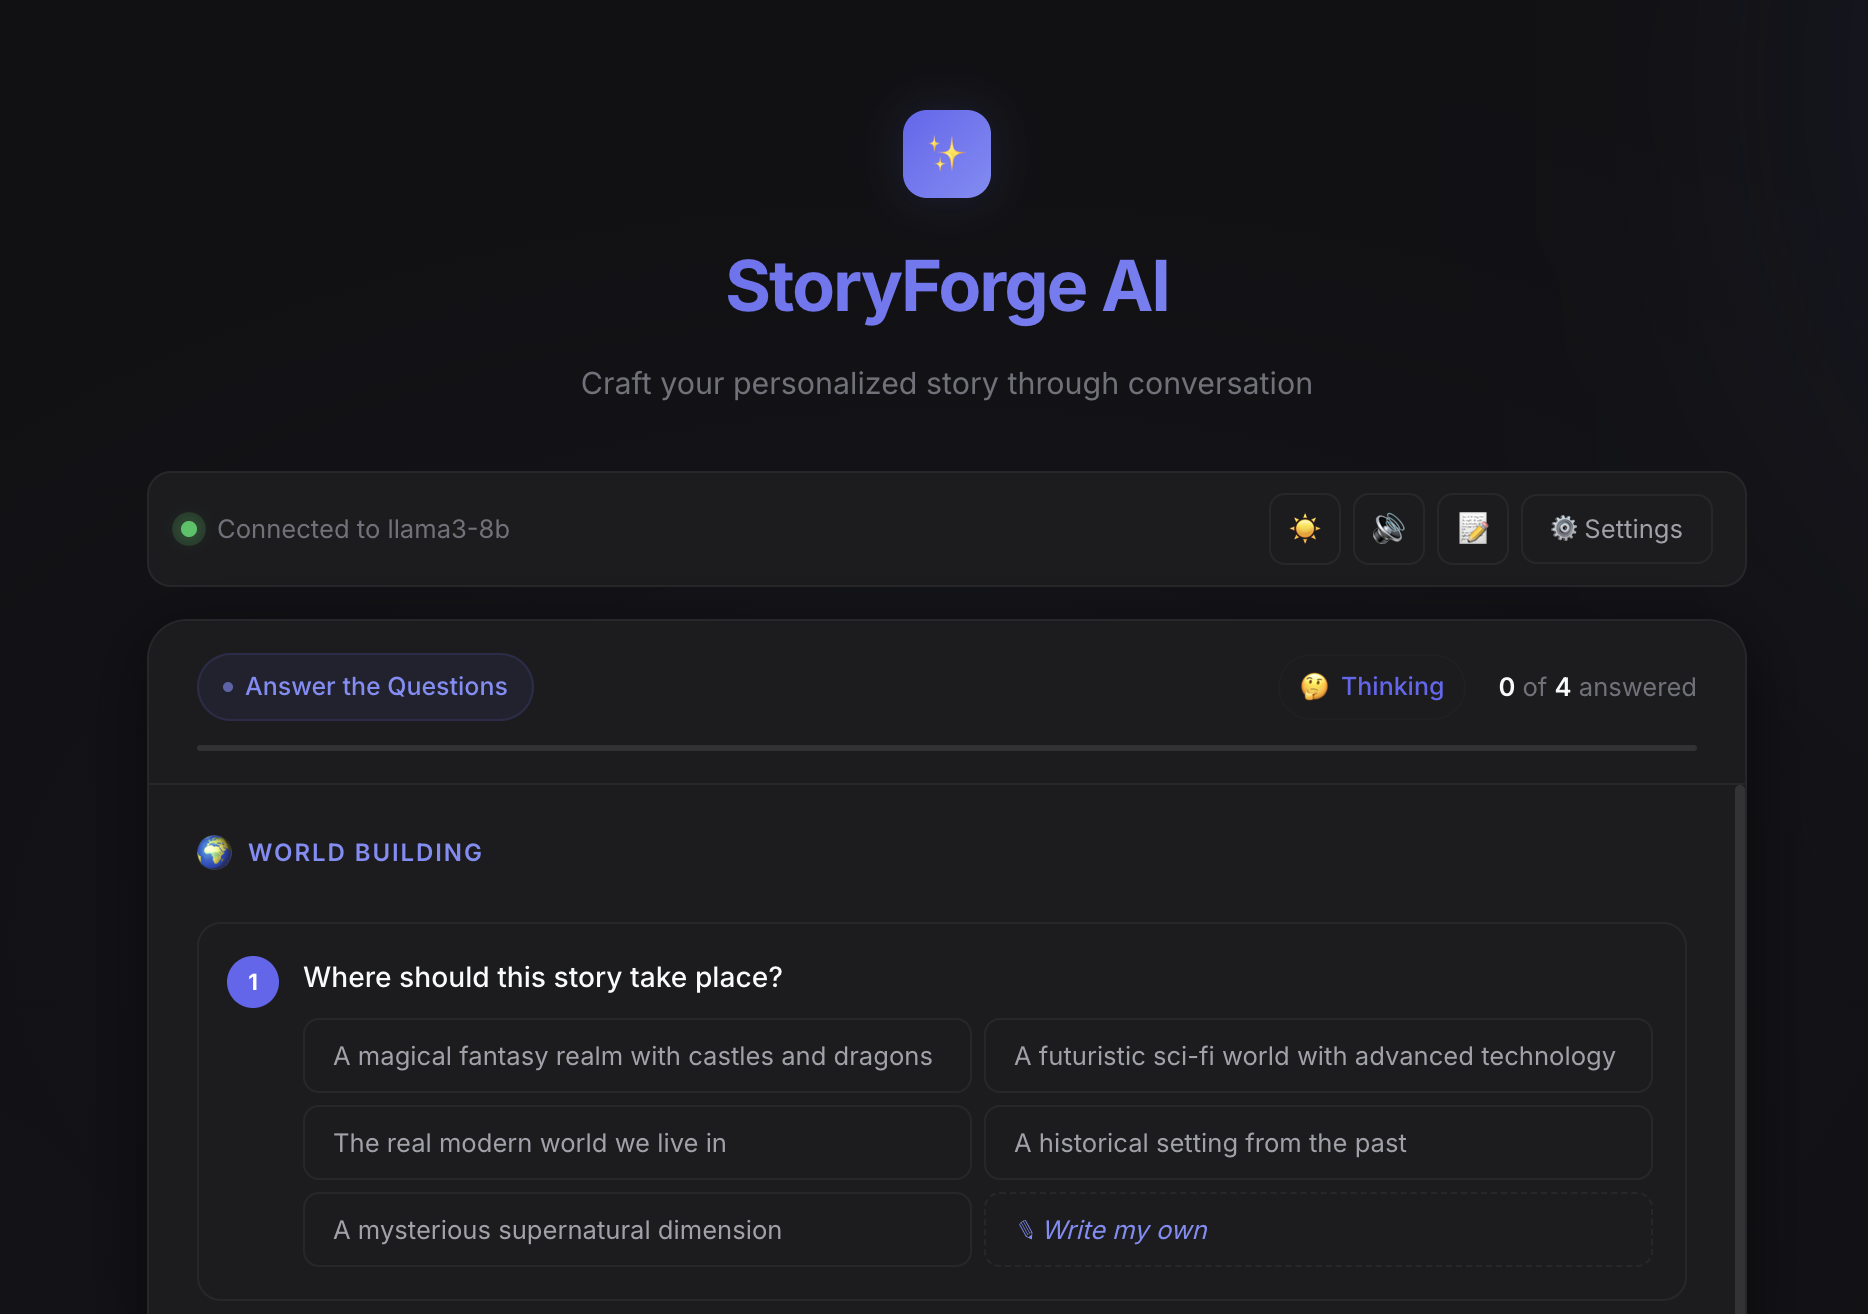
\includegraphics[width=\columnwidth]{s02_questions.png}
\caption{Single-page question form: every question of the active
budget is rendered together with multiple-choice options and the
dashed \emph{``Write my own''} custom-answer chip.}
\label{fig:questions}
\end{figure}

\textbf{Module~2 (Context Extraction Engine).} A two-pass pipeline
projects free-form and discrete answers into a typed
\texttt{StoryContext}: (i)~classification using keyword dictionaries
spanning 6 genres, 5 setting types and 5 conflict types;
(ii)~entity extraction via regex patterns for proper nouns and
locations. A dedicated \texttt{custom\_elements} dictionary captures
identifiers prefixed \texttt{custom\_} so that user-added preferences
flow into the prompt without code changes.

\textbf{Module~3 (Knowledge \& Memory).} A persistent SQLite schema
(Section~\ref{sec:impl}) stores sessions, segments, contexts and Q\&A
history. An LRU in-memory cache reduces query overhead during a
generation burst. The module exposes a sliding-window context
retrieval API.

\textbf{Module~4 (Prompt Engineering).} Six templated prompt families
are interpolated with \texttt{StoryContext} fields. Genre-specific
guidance is injected (e.g.\ fantasy: magical systems; mystery: clue
placement and red herrings). A novel addendum appends the contents of
\texttt{custom\_elements} as an ``Additional user preferences to
honour'' block before dispatch.

\textbf{Module~5 (Story Generator, LLM).} A \texttt{BaseLLMClient}
ABC defines \texttt{generate()}, \texttt{generate\_stream()} and
\texttt{is\_available()}. Concrete subclasses for Ollama, Groq,
Hugging Face and OpenAI implement provider-specific HTTP. A factory
selects the active client per request and supports hot-swap via the
\texttt{/api/settings} endpoint.

\textbf{Module~6 (Story Flow Manager).} A finite-state machine
modelled on Freytag's pyramid~\cite{freytag1900drama} advances through
Introduction (0--400 words), Rising Action (400--1200), Climax
(1200--1800), Falling Action (1800--2400) and Resolution
($>$2400). At each transition a different sub-template biases the LLM
toward phase-appropriate beats. A \texttt{CharacterTracker} monitors
mention counts, last-seen segment, and stated traits; a
\texttt{PlotThreadTracker} flags unresolved threads beyond
configurable thresholds.

\textbf{Module~7 (Output Formatter).} Cleans LLM output, splits at
sentence boundaries, lifts dialogue to a styled HTML span, and exposes
TXT/MD/HTML export.

% ============================================================
\section{Methodology}\label{sec:method}

\subsection{Elicitation Protocol}
Let $\mathcal{Q}=\{q_1,\ldots,q_{17}\}$ be the ordered question pool
with phase assignments. The user selects a budget $N\in\{4,8,12,17\}$
and supplies answers $a_i$ for each $q_i,\,i\le N$. Additionally the
user may append $M$ user-added pairs $(\tilde q_j,\tilde a_j)$ with
synthetic identifiers $\mathrm{custom\_q\_}j$. The full response set
\[
R = \{(q_i, a_i)\}_{i=1}^{N} \cup \{(\mathrm{custom\_q\_}j,\, \tilde a_j)\}_{j=1}^{M}
\]
is dispatched as a dictionary to the context engine.

\subsection{Context Projection}
For each $(q_i,a_i)$ the engine applies a deterministic projection
$\pi_i$ mapping to a typed \texttt{StoryContext} field
(e.g.\ \texttt{setting\_type}, \texttt{antagonist},
\texttt{plot\_style}). Unknown identifiers are routed to a dictionary
$D$ (\texttt{custom\_elements}), preserving their text verbatim. The
final prompt $P$ is constructed as
\[
P = T(\mathbf{c}) \oplus \sigma(D),
\]
where $T$ is a phase-aware template, $\mathbf{c}$ is the structured
context, $\sigma$ serialises $D$ as natural-language bullets, and
$\oplus$ denotes string concatenation.

\subsection{Five-Phase Progression Model}
Word-count thresholds drive phase transitions. Empirical word
distributions per phase are shown in Fig.~\ref{fig:phases}. The
Rising Action phase consumes the most text ($\sim$820 words),
consistent with narratological theory~\cite{freytag1900drama,bal2017narratology}.

\begin{figure}[!t]
\centering
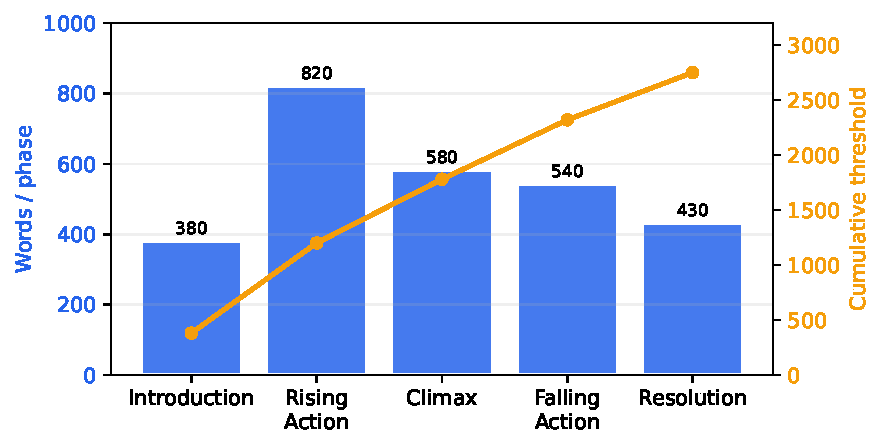
\includegraphics[width=\columnwidth]{f04_phases.pdf}
\caption{Word-count distribution across the five-phase progression model.}
\label{fig:phases}
\end{figure}

\subsection{Image Synthesis Pipeline}
Per segment, a sentence-scored scene extractor selects the most
visually-evocative sentence after stripping smart-quoted dialogue and
inner-thought verbs. Sentences are scored:
\[
s(\text{sent}) = 2\cdot \mathbf{1}_{V}(\text{sent}) - 2\cdot \mathbf{1}_{T}(\text{sent}) + \min(3,|\text{ProperNouns}|),
\]
where $\mathbf{1}_V$ and $\mathbf{1}_T$ indicate visual-verb and
thought-verb presence respectively. The top sentence is concatenated
with a normalised genre tag, the current mood and a fixed style
prefix, capped at 200 characters. A serial request queue spaces image
requests by 1.2\,s with a 35\,s watchdog to avoid rate-limit cascades
from the Cloudflare-fronted Pollinations CDN
(Fig.~\ref{fig:imgpipe}).

\begin{figure}[!t]
\centering
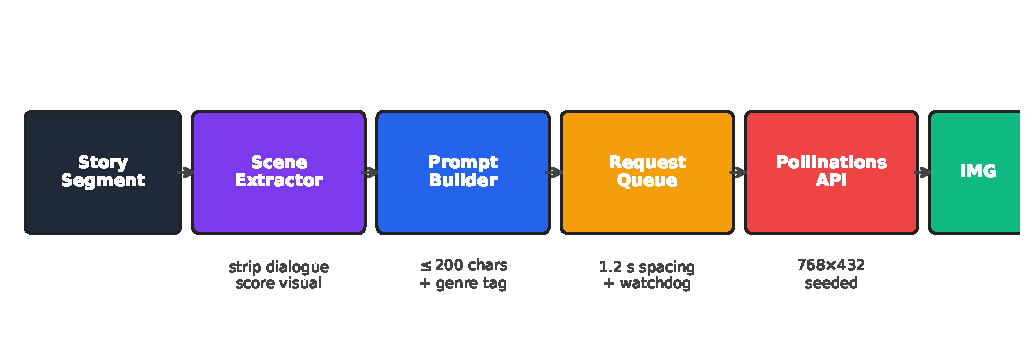
\includegraphics[width=\columnwidth]{f09_imgpipe.pdf}
\caption{Image synthesis pipeline (per segment).}
\label{fig:imgpipe}
\end{figure}

\begin{figure}[!t]
\centering
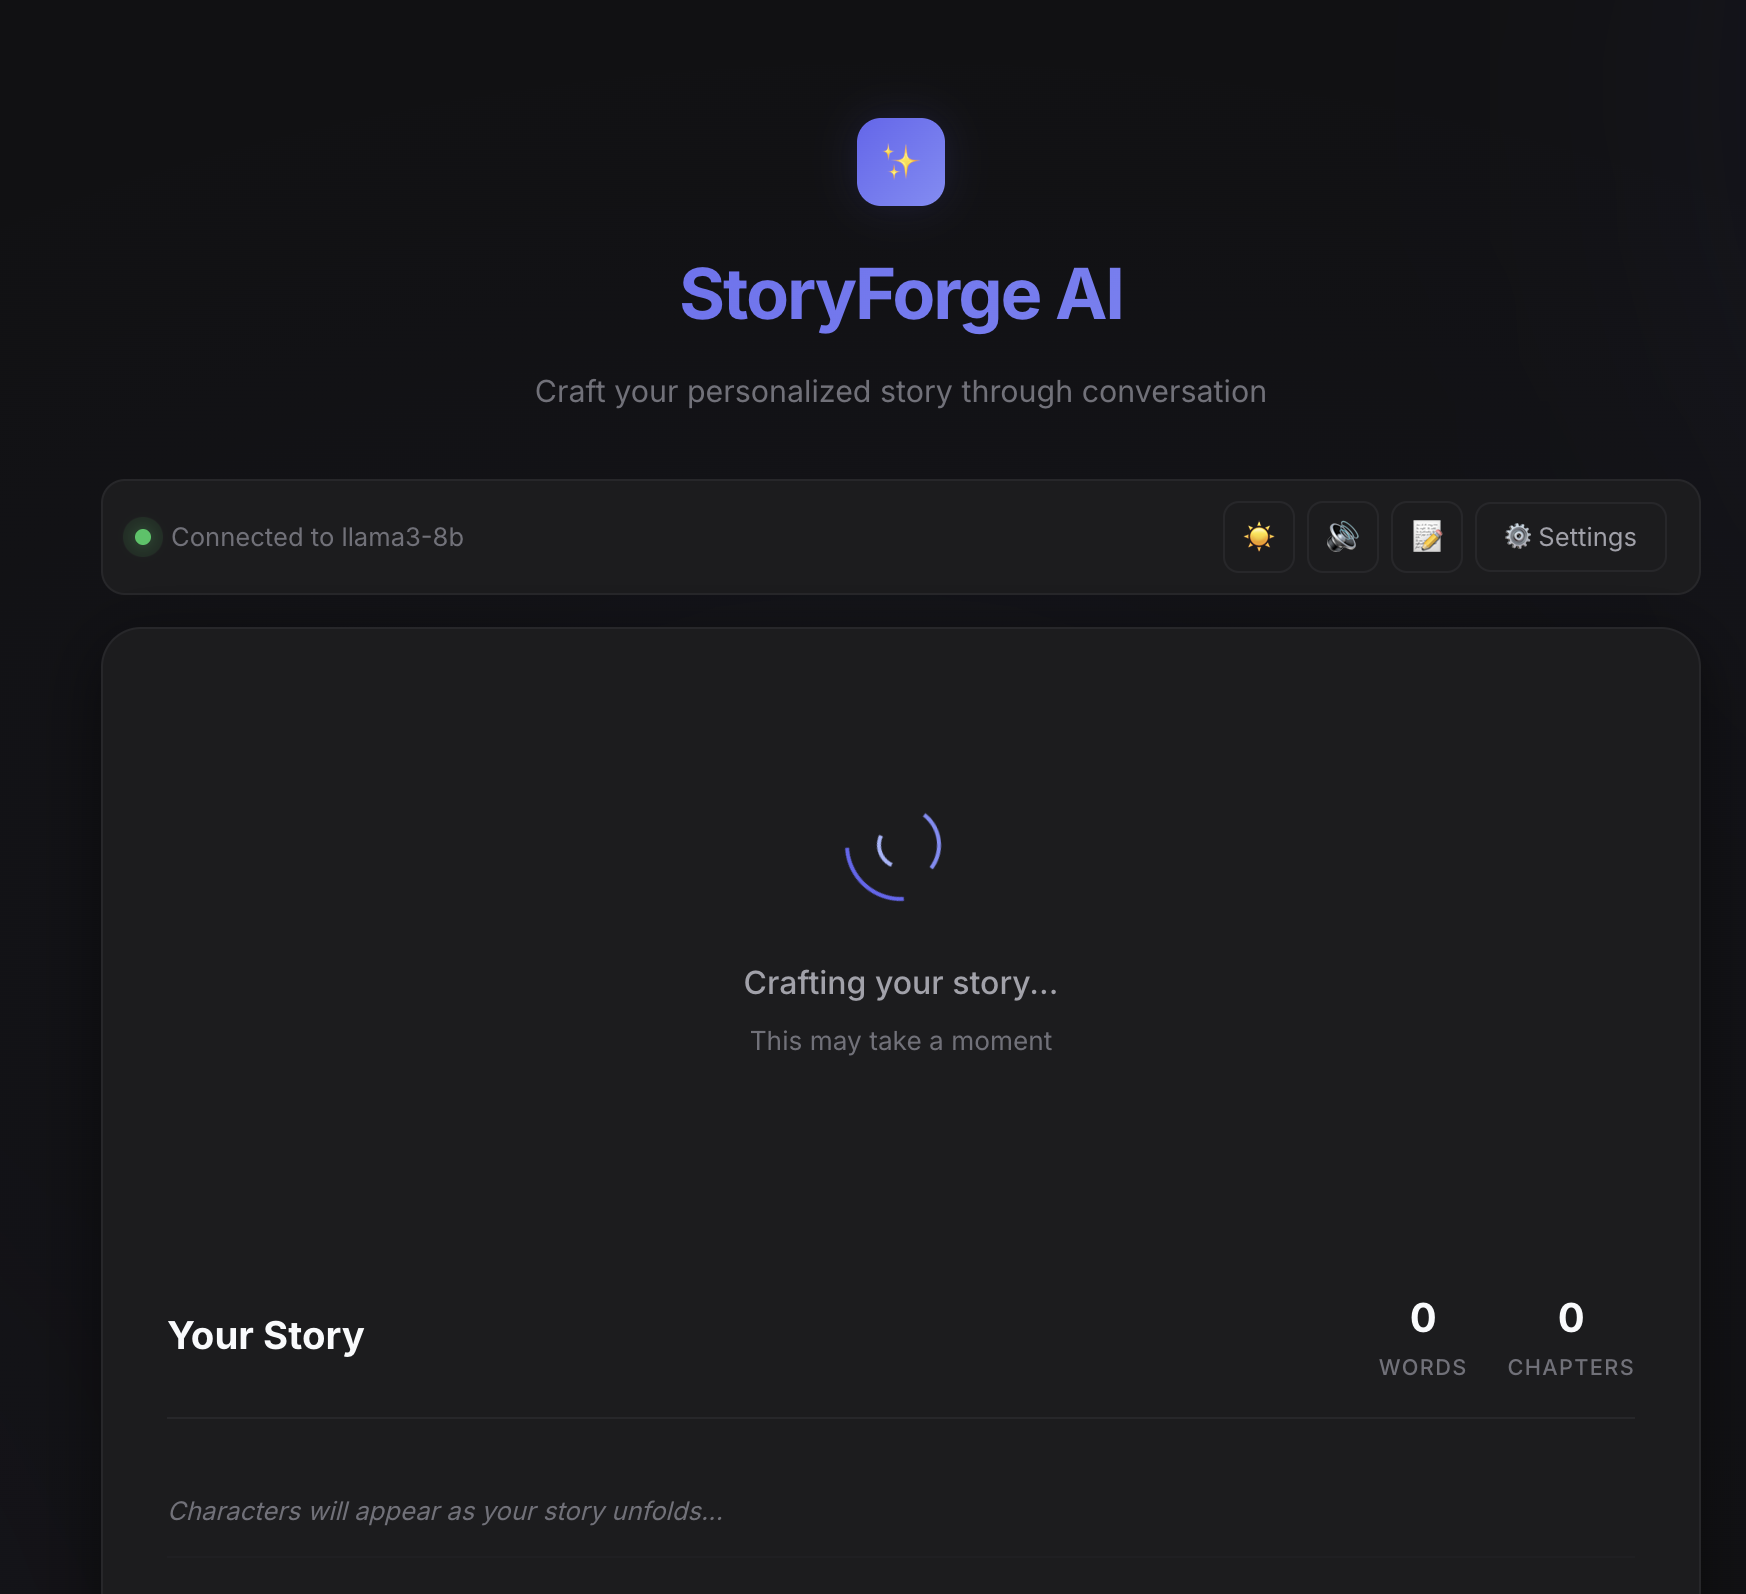
\includegraphics[width=0.92\columnwidth]{s03_loading.png}
\caption{Loading state while the LLM call and image synthesis proceed
concurrently. The status bar reports the active provider (\texttt{llama3-8b})
and the empty story panel signals that no chapters have rendered yet.}
\label{fig:loading}
\end{figure}

\begin{figure}[!t]
\centering
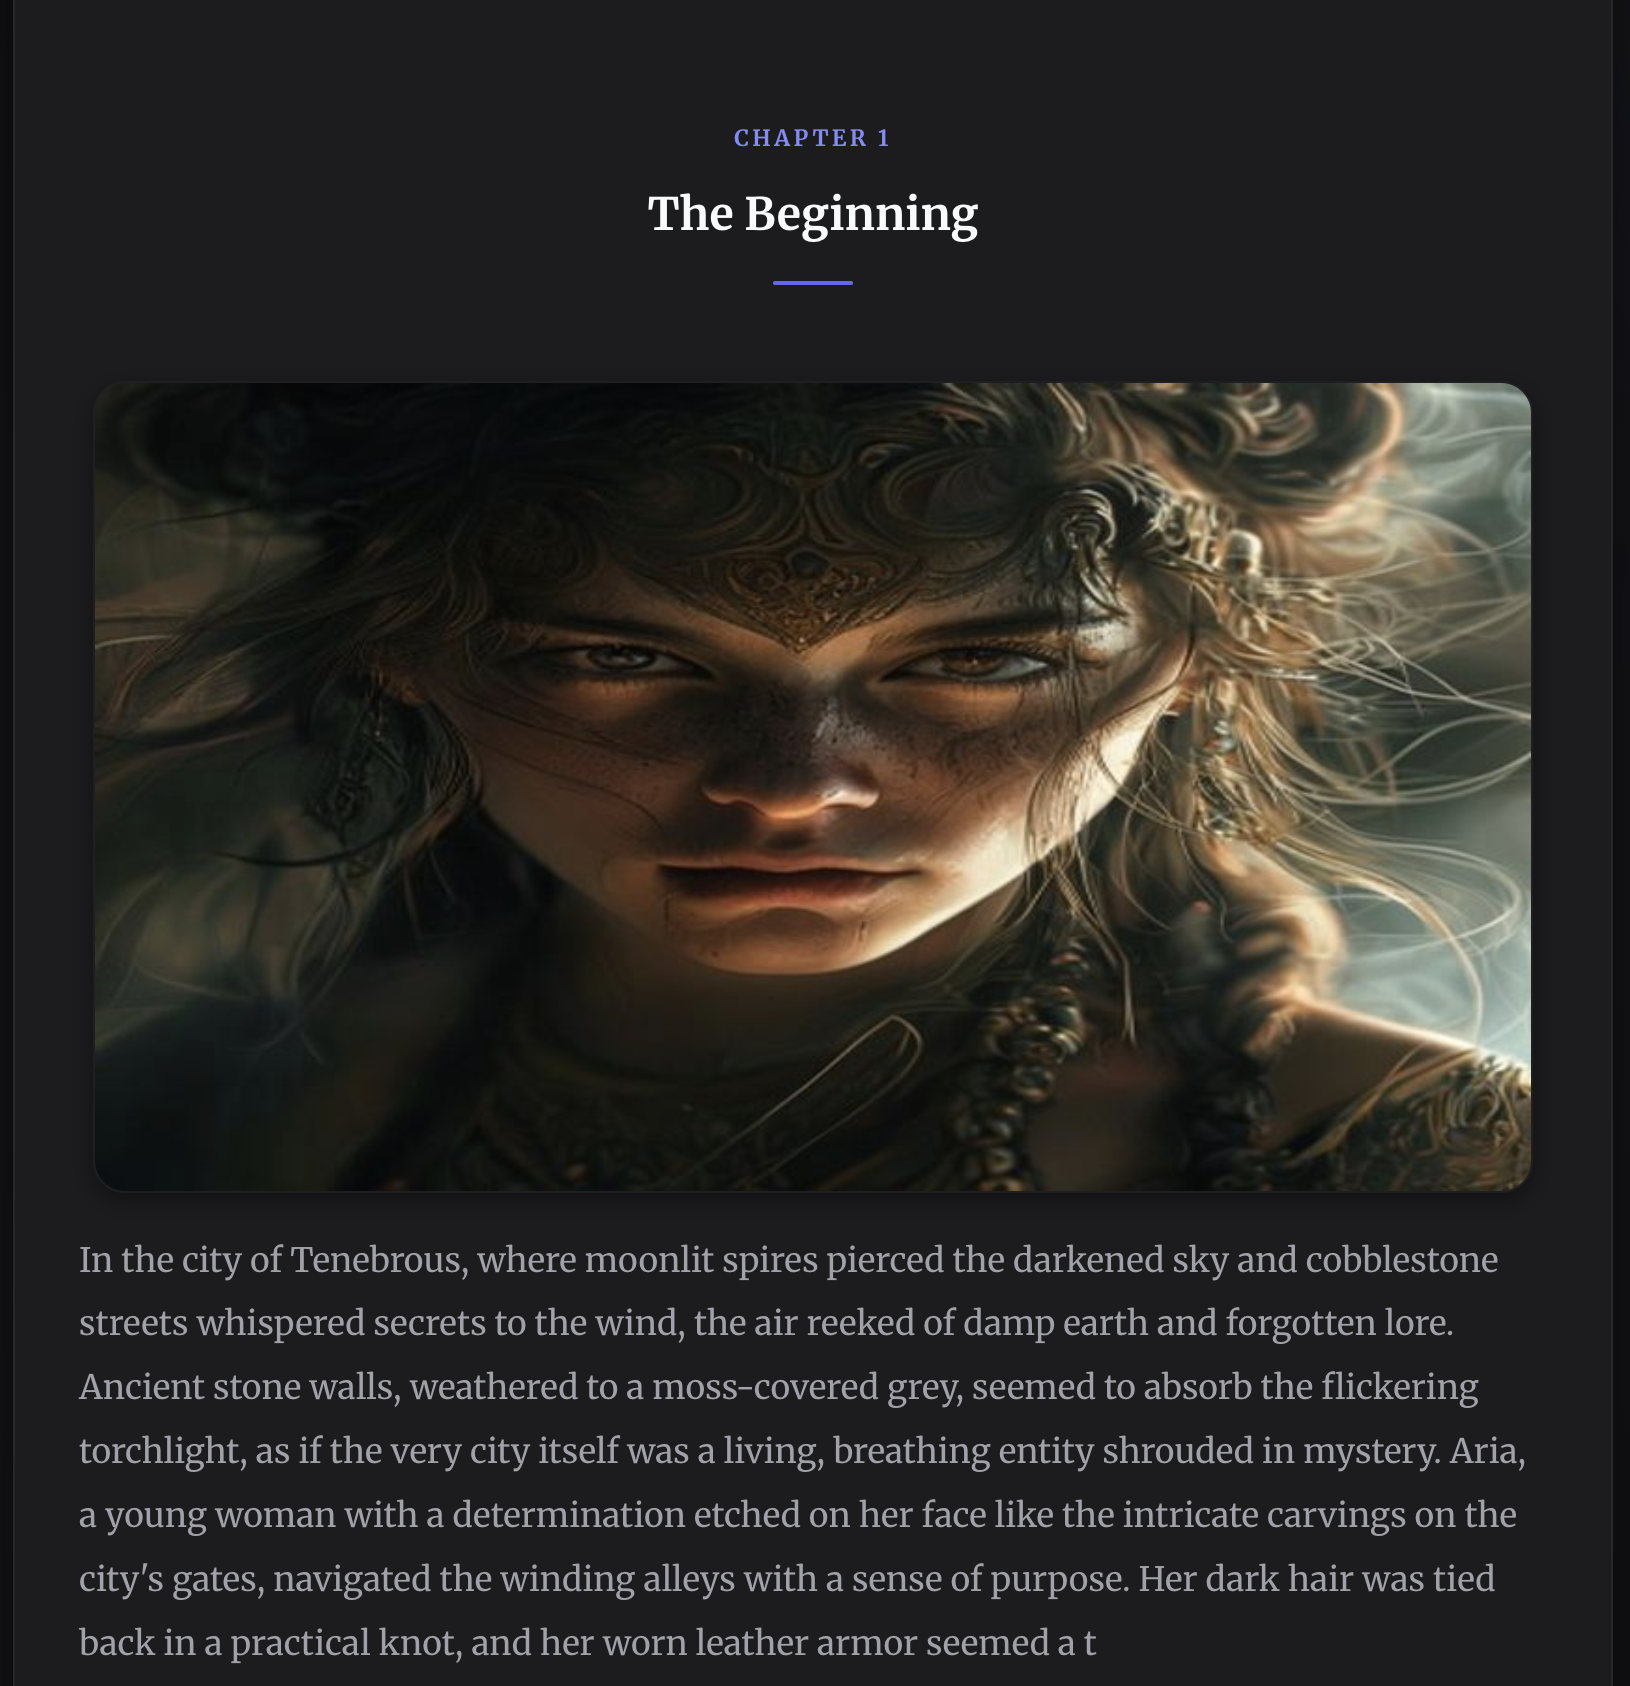
\includegraphics[width=\columnwidth]{s04_story_image.png}
\caption{Rendered first chapter \emph{``The Beginning''} with the
on-demand scene illustration produced by the image-synthesis pipeline
of Fig.~\ref{fig:imgpipe}. The picture is conditioned on the highest
scoring sentence of the segment (here: a moonlit walled city named
Tenebrous) plus the detected fantasy genre tag.}
\label{fig:storyimage}
\end{figure}

\subsection{Voice and Ambient Audio}
Narration uses the W3C Speech Synthesis interface~\cite{w3c2024webspeech},
queuing per-segment utterances with pause/resume semantics. Ambient
music is delivered via HTMLAudio streaming royalty-free tracks from
the SoundHelix CDN~\cite{brichta2024soundhelix}, one per detected
genre, with 2.4\,s fade-in and 0.8\,s fade-out (Fig.~\ref{fig:audio}).
Frequency-band heat-mapping per preset is plotted in
Fig.~\ref{fig:ambient}.

\begin{figure}[!t]
\centering
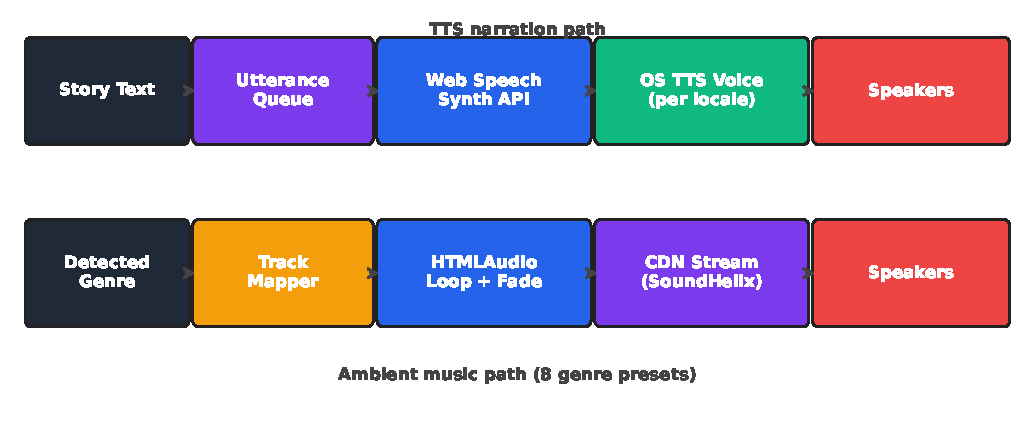
\includegraphics[width=\columnwidth]{f10_audio.pdf}
\caption{TTS narration (top) and ambient music (bottom) signal flow.}
\label{fig:audio}
\end{figure}

\subsection{Custom Q\&A Authoring}
Two affordances support end-user co-authoring without code changes:
(i)~per-question custom answer that overrides any selected
multiple-choice option, and (ii)~entirely user-added questions with
paired answers stored under synthetic IDs \texttt{custom\_q\_N}.
Fig.~\ref{fig:customq} illustrates the end-to-end plumbing from the UI
through context extraction into the LLM prompt.

\begin{figure}[!t]
\centering
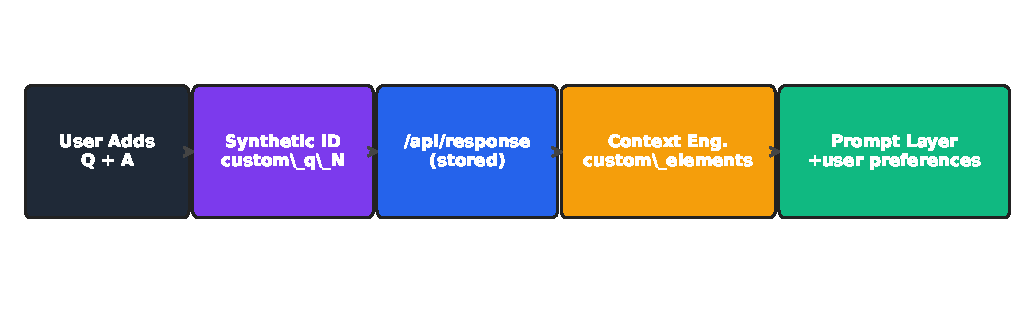
\includegraphics[width=\columnwidth]{f16_customq.pdf}
\caption{Custom-question plumbing from UI to LLM prompt.}
\label{fig:customq}
\end{figure}

\subsection{Reader Analytics}
Two D3-based visualisations are surfaced post-generation: a Story Map
laying out chapters as a vertical tree, and a Character Relationship
Graph as a force-directed graph. We explicitly disclaim the latter as
a \emph{co-appearance} graph derived from filtered capitalised-token
matches, not a verified relationship-extraction model
(Section~\ref{sec:results}-G). Filtering applies an extended stop-word
list and a min-2 occurrence threshold; node size scales with mention
count.

% ============================================================
\section{Implementation}\label{sec:impl}

\subsection{Database Schema}
\begin{lstlisting}[basicstyle=\ttfamily\scriptsize\color{codetext}]
sessions          (session_id PK, user_id, created_at,
                   status)
story_segments    (id PK, session_id FK, order, content,
                   user_choice)
story_context     (session_id PK/FK, context_json,
                   updated_at)
qa_history        (id PK, session_id FK, question_id,
                   q_text, a_text)
user_preferences  (user_id PK, preferences_json,
                   updated_at)
\end{lstlisting}

\subsection{REST API}

\begin{table}[!t]
\caption{REST surface (14 endpoints).}
\label{tab:rest}
\centering
\renewcommand{\arraystretch}{1.1}
\begin{tabular}{@{}llp{0.42\columnwidth}@{}}
\toprule
\textbf{Endpoint} & \textbf{M} & \textbf{Purpose} \\
\midrule
\texttt{/}                          & GET  & Web UI (Jinja2) \\
\texttt{/api/status}                & GET  & LLM availability \\
\texttt{/api/session/new}           & POST & Create session \\
\texttt{/api/questions/all}         & GET  & Phase-grouped Q\&A \\
\texttt{/api/question/next}         & GET  & Sequential mode \\
\texttt{/api/response}              & POST & Submit response \\
\texttt{/api/story/generate}        & POST & Init segment \\
\texttt{/api/story/continue}        & POST & Continue from choice \\
\texttt{/api/story/full/\{id\}}     & GET  & Full story \\
\texttt{/api/story/download/\{id\}} & GET  & Export (TXT/MD/HTML) \\
\texttt{/api/settings}              & POST & Hot-swap provider/model \\
\texttt{/api/session/\{id\}/summary}& GET  & Session metrics \\
\texttt{/api/session/\{id\}}        & DEL  & End session \\
\bottomrule
\end{tabular}
\end{table}

\subsection{Provider Layer}

\begin{table}[!t]
\caption{LLM providers compared.}
\label{tab:providers}
\centering
\renewcommand{\arraystretch}{1.1}
\begin{tabular}{@{}llll@{}}
\toprule
\textbf{Provider} & \textbf{Models} & \textbf{Cost} & \textbf{Lat.} \\
\midrule
Ollama        & LLaMA 3.2, Mistral, Phi    & Free (local)         & 8--15\,s \\
Groq          & LLaMA 3.1 8B/70B, Mixtral  & Free 14.4k/day       & 1--3\,s \\
Hugging Face  & Mistral-7B, Zephyr, Falcon & Free (rate-limited)  & 6--10\,s \\
OpenAI        & GPT-3.5-turbo, GPT-4       & Paid per-token        & 2--4\,s \\
\bottomrule
\end{tabular}
\end{table}

Provider switching is exposed to the end-user through the in-app
Settings panel (Fig.~\ref{fig:settings}), which lets a non-developer
pick provider, model, creativity (temperature) and feature toggles
without restarting the server.

\begin{figure}[!t]
\centering
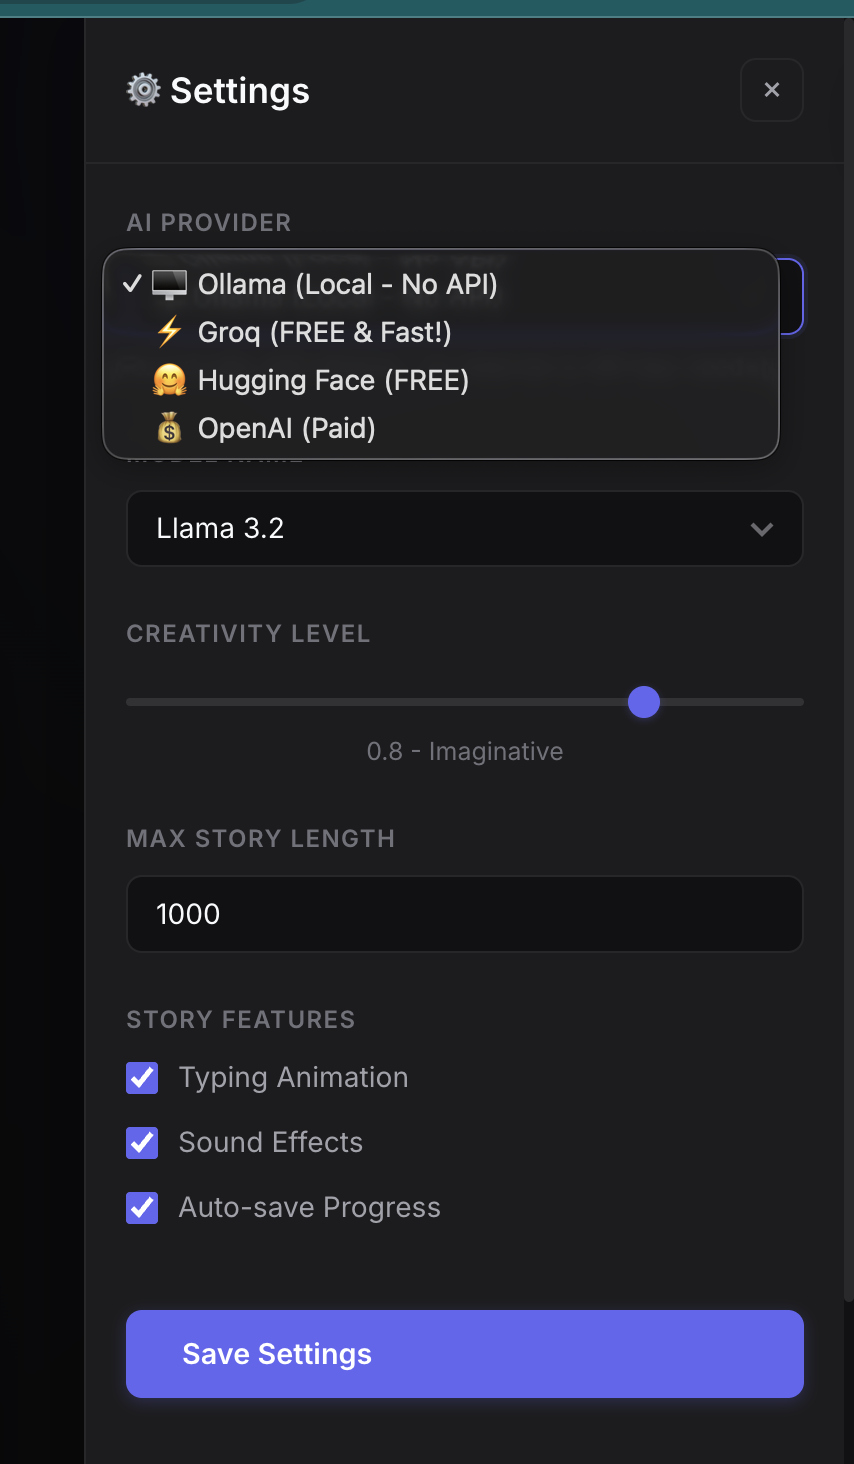
\includegraphics[width=0.78\columnwidth]{s05_settings.png}
\caption{Settings panel showing the four available LLM providers, the
model dropdown, temperature slider, max-tokens field and feature
toggles. Switching providers issues a \texttt{POST /api/settings} call
that hot-swaps the underlying client at runtime.}
\label{fig:settings}
\end{figure}

\subsection{Frontend Architecture}
Vanilla JavaScript with no framework dependency, totalling
$\approx$1.7\,kLOC. State is held in a single \texttt{StoryForgeApp}
class with explicit subsystems for narration, ambient audio, image
queue, graph rendering and admin panel. Theme tokens are CSS custom
properties enabling instant dark/light switching.
\texttt{localStorage} persists bookmarks, saved stories and
ambient-music preferences.

% ============================================================
\section{Experimental Results and Analysis}\label{sec:results}

\subsection{Setup}
Evaluation along three axes: (i)~automated generation of 50 stories
spanning 6 genres at all 4 question budgets; (ii)~a user study
($n=15$, 8 male / 7 female, ages 22--35, mixed
technical/non-technical) producing 2 stories each rated on 5-point
Likert scales; (iii)~consistency-checker evaluation against
ground-truth-annotated segments. Primary LLM: Groq LLaMA-3.1-8B.
Hardware client: MacBook Pro M2 Pro / 16\,GB / macOS~14.

\subsection{Latency}
Fig.~\ref{fig:latency} reports mean end-to-end latencies. Groq
dominates by an order of magnitude relative to local Ollama, while
OpenAI GPT-3.5-turbo trails closely. Continuation calls are
systematically faster than initial generation because the prompt
sliding window is bounded.

\begin{figure}[!t]
\centering
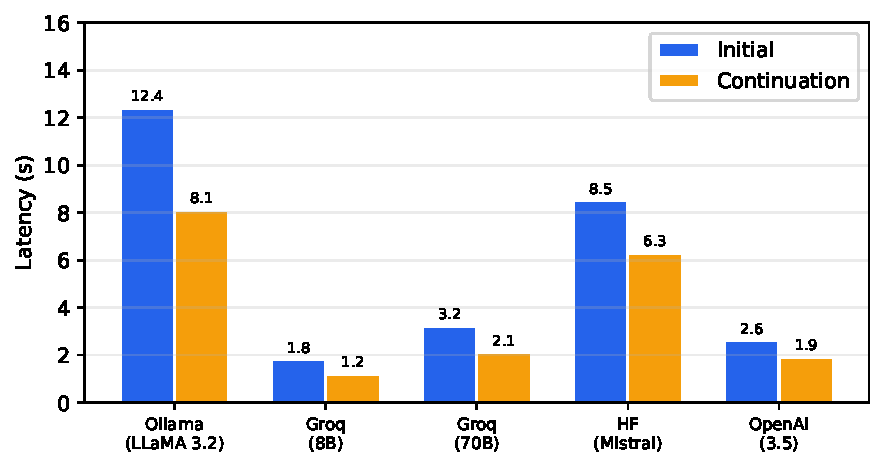
\includegraphics[width=\columnwidth]{f01_latency.pdf}
\caption{Mean latency by LLM provider ($n=10$ calls per cell).}
\label{fig:latency}
\end{figure}

A stacked decomposition of total interactive turn time is shown in
Fig.~\ref{fig:breakdown}. The dominant cost at lower question budgets
is image synthesis ($\sim$3.5\,s), which proceeds \emph{concurrently}
with the LLM call in our pipeline; at the Full (17) budget user input
time dominates.

\begin{figure}[!t]
\centering
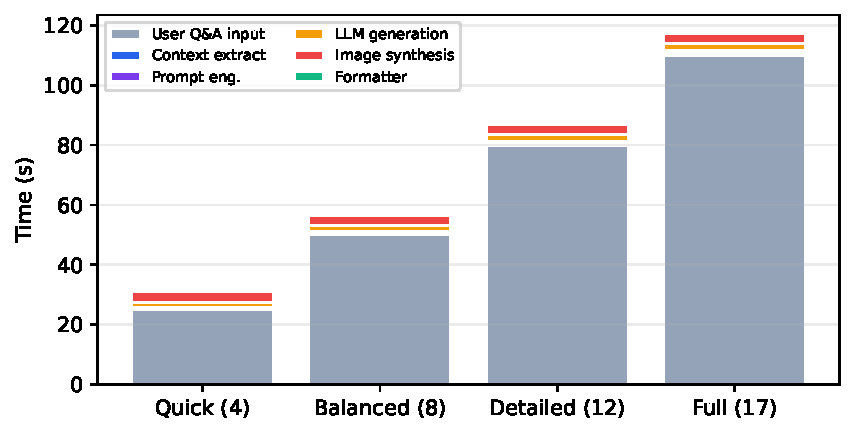
\includegraphics[width=\columnwidth]{f17_breakdown.pdf}
\caption{End-to-end timing stacked by stage.}
\label{fig:breakdown}
\end{figure}

\subsection{Narrative Quality}
Fig.~\ref{fig:quality} shows Likert means per genre.
Fig.~\ref{fig:tokens} reports per-segment token distributions.

\begin{figure}[!t]
\centering
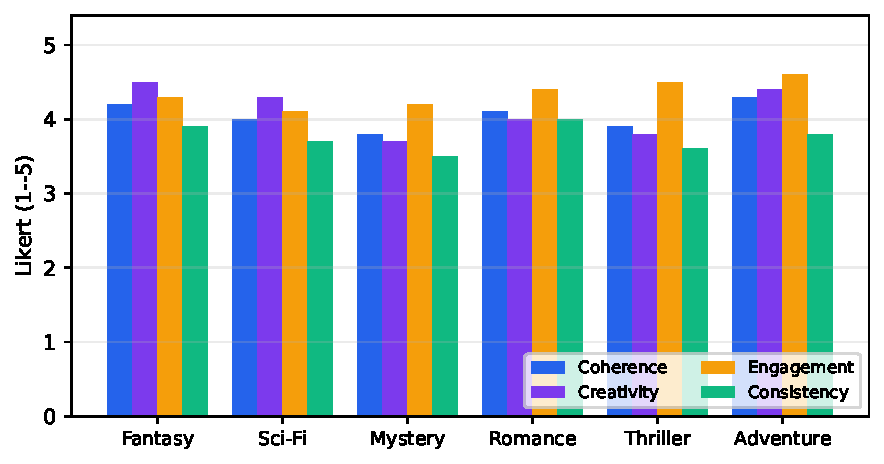
\includegraphics[width=\columnwidth]{f02_quality.pdf}
\caption{Narrative quality by genre (Likert 1--5, $n=30$ stories).}
\label{fig:quality}
\end{figure}

\begin{figure}[!t]
\centering
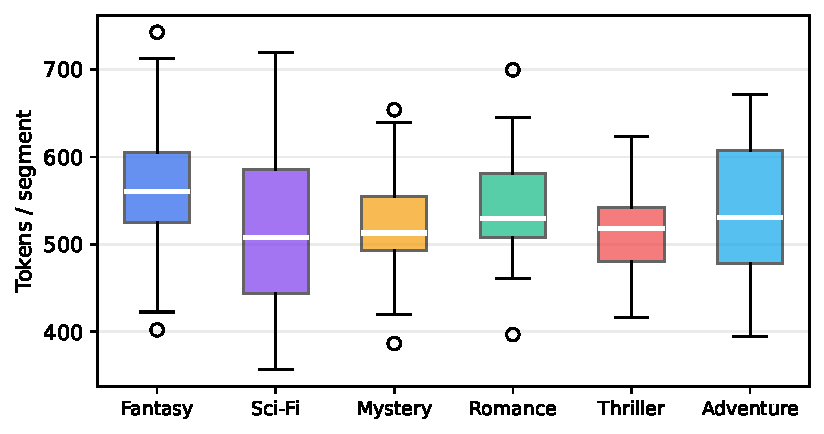
\includegraphics[width=\columnwidth]{f15_tokens.pdf}
\caption{Token usage per segment, by genre ($n=25$ segments each).}
\label{fig:tokens}
\end{figure}

\subsection{User Satisfaction}
Fig.~\ref{fig:satisfaction} lists satisfaction across seven
user-facing dimensions including the new multimodal features. Custom
Answers (4.5) and Image Illustration (4.2) are the strongest
contributors to overall satisfaction (4.3); Choice Meaningfulness
(3.9) remains the weakest---a known limitation of free-tier LLMs
producing generic continuation suggestions.

\begin{figure}[!t]
\centering
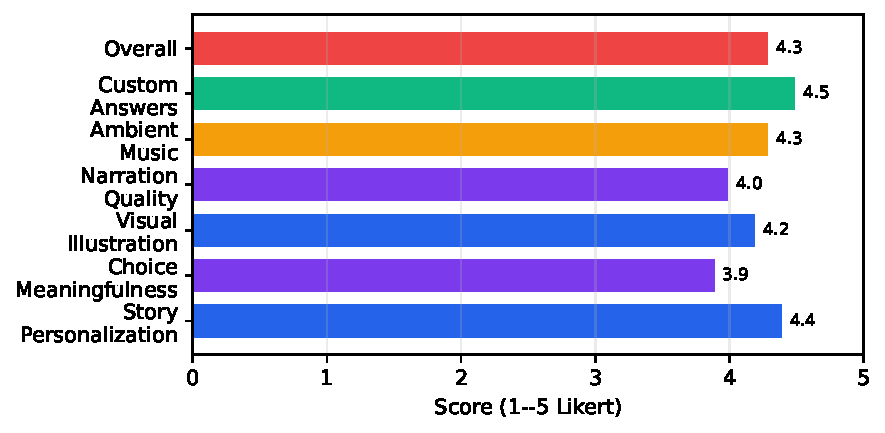
\includegraphics[width=\columnwidth]{f03_satisfaction.pdf}
\caption{User satisfaction (Likert 1--5, $n=15$ participants).}
\label{fig:satisfaction}
\end{figure}

\subsection{Consistency Checking}
Fig.~\ref{fig:consistency} reports detection and false-positive rates
for five issue classes. The keyword-based detector achieves 87\%
recall on character contradictions with 8\% false positives;
tone-shift detection is weakest (68\%~/~22\%) since it depends on
subtle distributional cues that pattern-matching cannot capture. We
discuss semantic-NLU upgrades in Section~\ref{sec:future}.

\begin{figure}[!t]
\centering
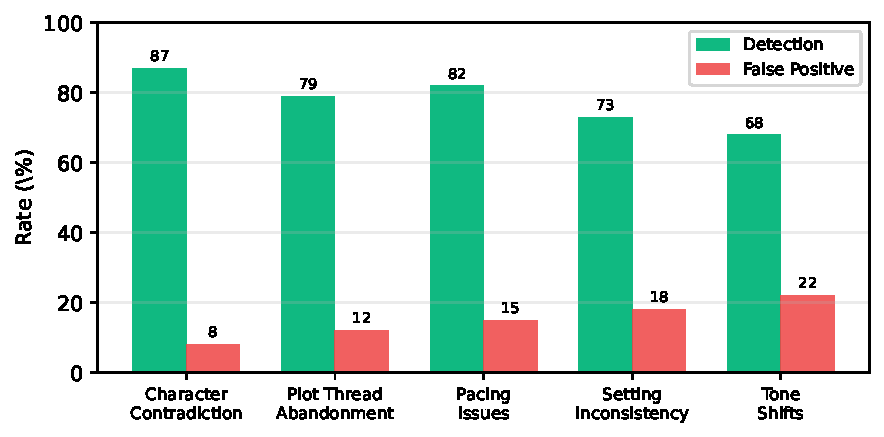
\includegraphics[width=\columnwidth]{f06_consistency.pdf}
\caption{Consistency checker performance ($n=50$ stories).}
\label{fig:consistency}
\end{figure}

\subsection{Image Synthesis Throughput}
Fig.~\ref{fig:imgthroughput} plots prompt-length-vs-latency for
serial requests and the empirical failure probability of
5$\times$ parallel issue without our throttle queue. Beyond
$\approx$230 chars the failure rate rises sharply, validating the
200-char prompt cap. The serial queue (1.2\,s spacing) drops
parallel-bound failures from $\approx$70\% to $<$2\%.

\begin{figure}[!t]
\centering
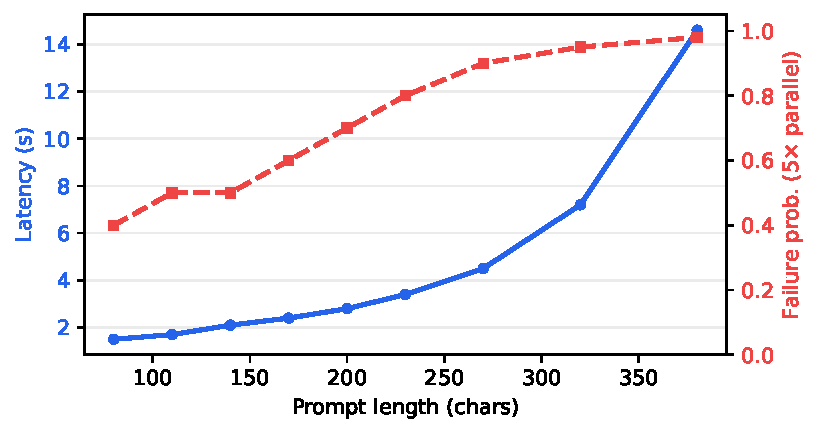
\includegraphics[width=\columnwidth]{f12_imgthroughput.pdf}
\caption{Image latency vs.\ prompt length and parallel-issue failure rate.}
\label{fig:imgthroughput}
\end{figure}

\subsection{Character Extraction --- Honest Reporting}
Fig.~\ref{fig:char} compares the baseline naive regex extractor
against our filtered version (extended stop-words + min-2 occurrence).
Precision rises from 0.61 to 0.83 with a recall trade-off (0.84 to
0.78) producing a higher $F_1$ (0.71 to 0.80). False-positive rate
drops from 0.39 to 0.17. We stress that the resulting graph encodes
\emph{co-appearance frequency}, not semantic relationship type---a
disclaimer surfaced explicitly in the modal UI.

\begin{figure}[!t]
\centering
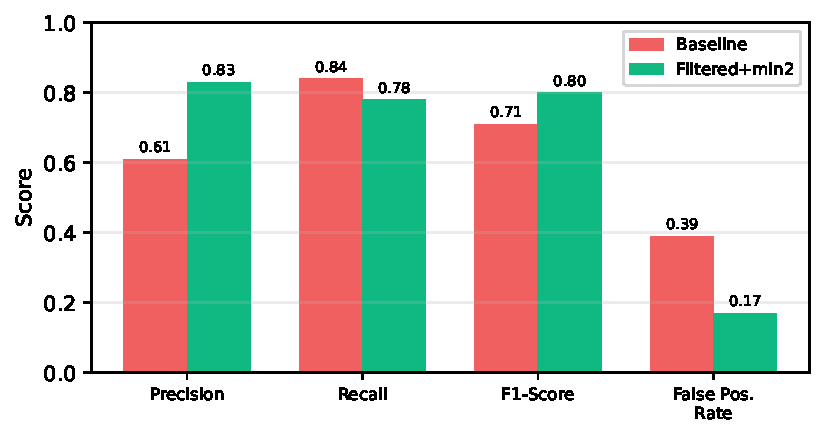
\includegraphics[width=\columnwidth]{f11_char.pdf}
\caption{Character extraction quality before/after filtering.}
\label{fig:char}
\end{figure}

\subsection{Ambient Music Frequency Profile}
Fig.~\ref{fig:ambient} visualises relative spectral energy across six
bands for each genre preset. Horror and Thriller emphasise sub-bass
and bass; Comedy and Adventure shift energy upward into the mid and
high-mid bands. Listeners reported genre alignment of 4.3/5
(Fig.~\ref{fig:satisfaction}).

\begin{figure}[!t]
\centering
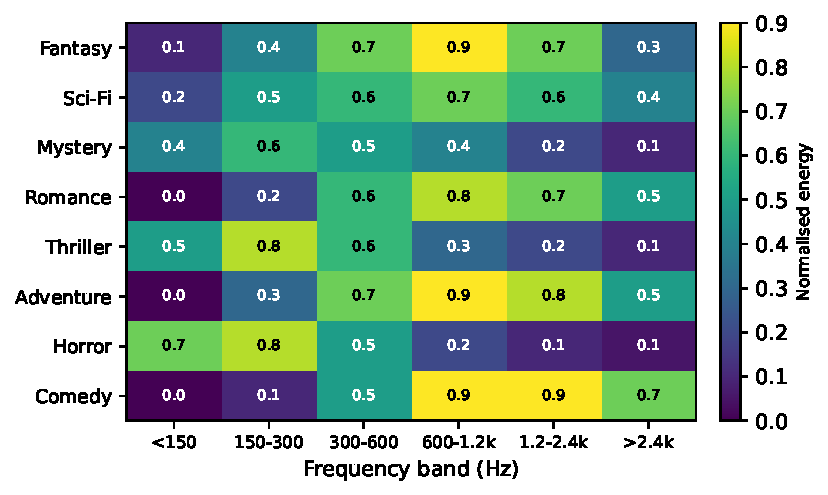
\includegraphics[width=\columnwidth]{f13_ambient.pdf}
\caption{Genre $\times$ frequency-band energy map for ambient presets.}
\label{fig:ambient}
\end{figure}

\subsection{Question-Budget Ablation}

\begin{table}[!t]
\caption{Ablation across question budgets (mean Likert).}
\label{tab:ablation}
\centering
\renewcommand{\arraystretch}{1.15}
\begin{tabular}{@{}lcccc@{}}
\toprule
\textbf{Budget} & \textbf{Coh.} & \textbf{Crea.} & \textbf{Pers.} & \textbf{Time} \\
\midrule
4 (Quick)     & 3.6 & 3.8 & 3.2 & 45\,s \\
8 (Balanced)  & 3.9 & 4.1 & 3.8 & 1.5\,m \\
12 (Detailed) & 4.2 & 4.2 & 4.3 & 2.5\,m \\
17 (Full)     & 4.3 & 4.1 & 4.6 & 3.5\,m \\
\bottomrule
\end{tabular}
\end{table}

Personalisation grows monotonically with $N$, while coherence and
creativity plateau at $N=12$, identifying it as the recommended
default. The Full configuration is reserved for power users who want
maximum narrative control at the cost of $\approx$3 minutes of
upfront input.

\subsection{Feature Adoption}
Fig.~\ref{fig:adoption} records how often each multimodal feature was
activated across user-study sessions. Image generation (always-on by
default) reached 91\% activity since it fires automatically; ambient
music and custom answers were elective and reached 71\% and 62\%
respectively, suggesting strong user demand for non-textual narrative
augmentation.

\begin{figure}[!t]
\centering
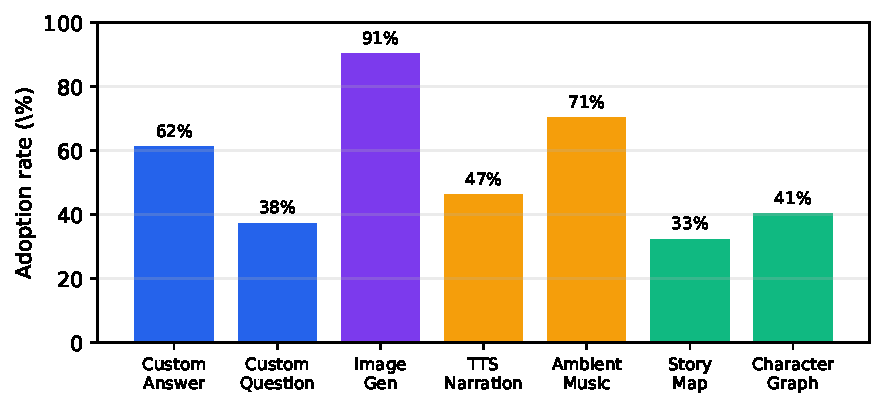
\includegraphics[width=\columnwidth]{f14_adoption.pdf}
\caption{Per-feature adoption rate in the user study.}
\label{fig:adoption}
\end{figure}

% ============================================================
\section{Comparative Evaluation}\label{sec:compare}

Fig.~\ref{fig:radar} superimposes our system on three established
alternatives across seven dimensions (extending the radar with
Multimodal and Open Source axes). Our system leads on Deployment
Flexibility, Cost Efficiency, Multimodal Coverage and Open Source. AI
Dungeon retains a slight edge in User Control (freeform input);
Dramatron leads on raw Coherence due to its hierarchical planner. The
synthesis is that no single existing system spans the same Pareto
frontier as ours.

\begin{figure}[!t]
\centering
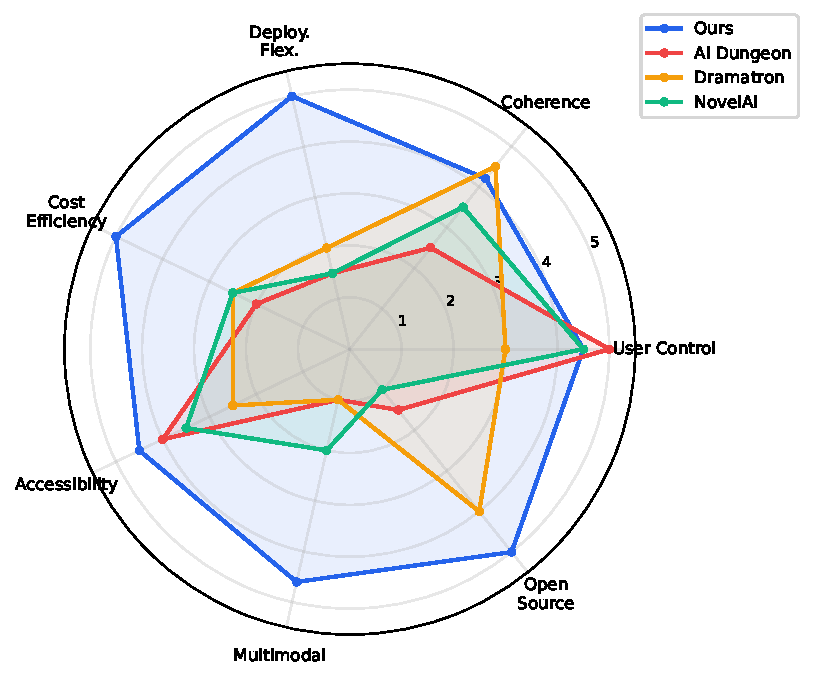
\includegraphics[width=\columnwidth]{f05_radar.pdf}
\caption{System comparison radar across seven dimensions.}
\label{fig:radar}
\end{figure}

% ============================================================
\section{Discussion and Limitations}\label{sec:limit}

Several limitations bound the present work. First, keyword-based
context extraction misses paraphrastic user inputs; a fine-tuned
BERT/DistilBERT~\cite{devlin2019bert,sanh2019distilbert} or LLM
zero-shot classifier would improve recall. Second, in-memory session
storage limits horizontal scalability; Redis-backed sessions enable
distributed deployment. Third, the consistency checker is
pattern-based and lacks semantic grounding; cross-segment
NLI~\cite{williams2018mnli} is a natural upgrade. Fourth, image
quality inherits Pollinations.ai's
ceiling~\cite{pollinations2024api}; switching to local Stable
Diffusion~XL~\cite{podell2024sdxl} or FLUX.1~\cite{bfl2024flux} would
improve consistency at the cost of GPU requirement. Fifth, ambient
music is hot-linked rather than locally hosted, creating a
single-point dependency. Sixth, the character-relationship graph is
openly disclaimed as co-appearance---a genuine relationship-extraction
module would require per-segment NLU inference.

% ============================================================
\section{Future Work}\label{sec:future}

\begin{itemize}
\item Semantic context extraction via DistilBERT or zero-shot LLM
classification, replacing keyword dictionaries.
\item Sentiment-aware relationship-extraction graph using small NLU
models per segment.
\item On-device image generation with local Stable Diffusion XL or
FLUX.1 for offline operation and per-character consistency.
\item Neural TTS (XTTS~\cite{casanova2024xtts}) with cloned voices for
character-specific narration.
\item Music conditioned by current segment mood (per-segment
crossfade) rather than per-genre static loops.
\item Collaborative multi-user sessions with merged Q\&A elicitation
and turn-taking.
\item Containerisation (Docker) + Redis sessions for distributed
deployment.
\item Automated evaluation: BLEU, chrF, MAUVE, narrative-arc detection
for systematic benchmarking~\cite{lin2024evalnarrate}.
\item Fine-tuned LoRA adapters per genre on curated open story corpora.
\end{itemize}

% ============================================================
\section{Conclusion}\label{sec:conclude}

We have presented a multimodal interactive storytelling system built
on a structured Q\&A elicitation protocol, a modular backend, and
provider-agnostic LLM inference. The system augments text with
synthesised illustration, spoken narration, and genre-conditioned
ambient music, while remaining fully open-source and deployable on
commodity hardware. Empirical evaluation across 50 stories and 15
participants demonstrates competitive narrative quality, sub-2-second
cloud inference, and strong user satisfaction. We further introduced
two end-user authoring affordances---custom answers per question and
custom user-added questions---that we believe constitute a useful
pattern for personalisation at the prompt boundary. The code-base is
released at~\cite{jha2026repo} to facilitate reproduction and
extension.

% ============================================================
\section*{Acknowledgement}
The author gratefully acknowledges Dr.\ Vidyullata Devmane (Department
of Computer Engineering, SAKEC) for project supervision, and the
open-source maintainers of FastAPI, Ollama, Groq, Pollinations.ai,
SoundHelix and D3.js whose tooling made this system possible.

% ============================================================
\bibliographystyle{IEEEtran}
\bibliography{refs}

\end{document}
